\section{Results}\label{sec:results}

\subsection{Sigma Hyperparameter Selection}\label{subsec:sigmaHyperparameterSelectionResults}
Recall that $\sigma_1, \sigma_2, \ldots \sigma_n$ are hyperparameters that must be defined prior to executing the
algorithm.
The grid search exhausts every permutation $P_n^{\sigma_n}$, where:
\begin{equation}
    \label{eq:gridSearchQuerySigma}
    \sigma_n \ \in \ \{10^{-16}, 10^{-15}, \ldots 10^{1}\}
\end{equation}
% 2.22 * 10^-16 is the machine epsilon for double

\begin{figure*}
    \centering{
    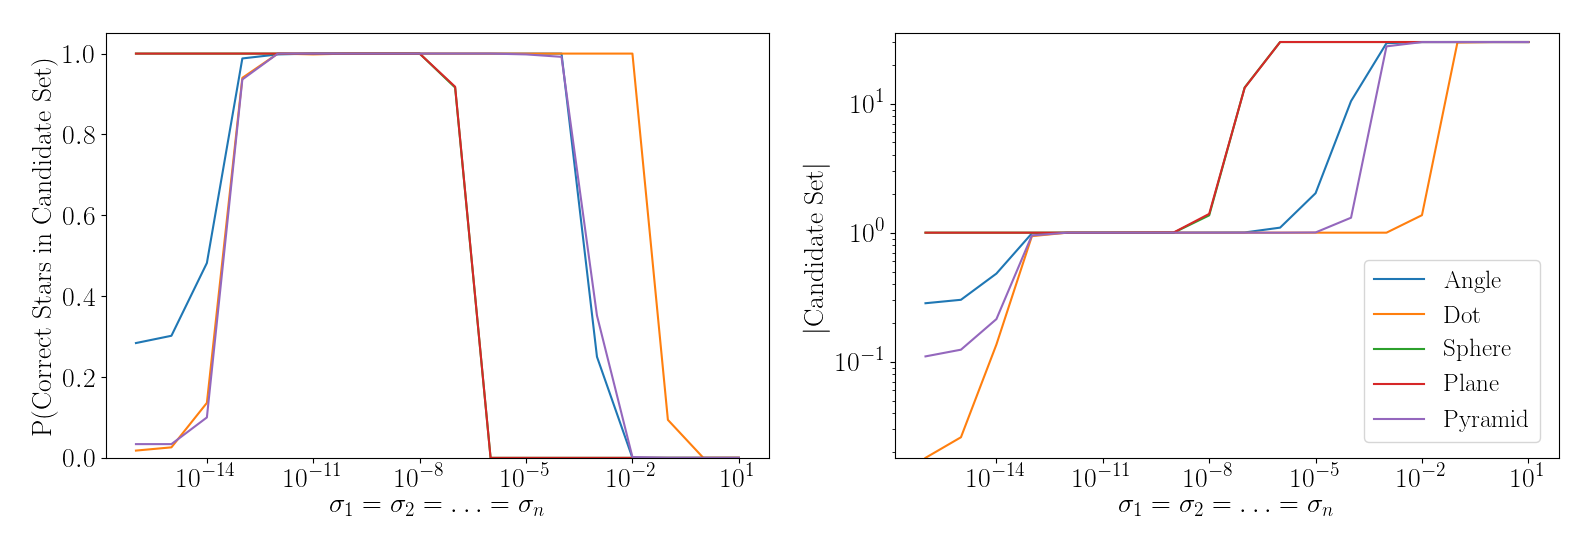
\includegraphics[scale=0.45]{images/sigma1-pcss-css.png}
    \caption{
    The left plot depicts the effect of varying $\sigma$ on the probability that the correct star set exists in the
    resulting candidates after the query.
    The right plot depicts the effect of varying $\sigma$ on the average size of the candidate set after the query, bounded
    by 30 candidates at maximum.
    The field-of-view is bounded by $f = 20^\circ$ and the apparent magnitude is bounded by $m = 6.0$.
    Each point represents the average of 1000 query steps without noise introduced.
    For brevity, all deviations associated with methods of more than one feature term (i.e.\ Dot Angle, Spherical
    Triangle, \ldots) had all corresponding $\sigma$ terms set equal to each other.
    } \label{figure:sigmaHyperparameterPlots}
    }
\end{figure*}

The set of plots in~\autoref{figure:sigmaHyperparameterPlots} depict the effect on different $\sigma$ terms against the
average size of the candidate set $S$ (on the left) and the probability that the correct stars exist in this candidate
set $Q$ (on the right).
If the deviation is too small, then the selectivity of each query becomes too restrictive and no results are returned.
On the other hand when the selectivity is too high, the candidate set size upper bound of 30 candidates is
hit and the chance that the correct candidate exists in the query declines.

The ideal period for all methods identifying images restricted by $f < 20 \land m < 6.0$ occurs when:
\begin{equation}
    \label{eq:idealRegionAcrossFeatures}
    \sigma_n \ \in (10^{-12}, 10^{-8})
\end{equation}
Regardless of the feature, a deviation choice between these bounds should be acceptable for distinguishing stars.

% Not including this, don't feel it is relevant to ideal analysis.
%It is important to note that each feature exists in different bounds.
%The values below represent the observed bounds of each feature:
%\begin{alignat*}{2}
%    \label{eq:observedFeatureSpace}
%    % Non-inclusive bounds given below.
%    \theta^{ij} &\in (2.6 \times 10^{-3} &&, 2.0 \times 10^1) \\
%    \theta^{ij} &\in  (2.6 \times 10^{-3} &&, 2.0 \times 10^1) \\
%    \theta^{ic}, \theta^{jc} &\in (2.6 \times 10^{-3} &&, 2.0 \times 10^1) \\
%    \phi &\in (1.3 \times 10^{-3} &&, 1.8 \times 10^2) \\
%    a^{ijk} &\in (3.1 \times 10^{-9} &&, 5.4 \times 10^{-2}) \\
%    \imath^{ijk} &\in (4.8 \times 10^{-16} &&, 5.3 \times 10^{-4}) \\
%    a^{ijk} &\in (3.7 \times 10^{-9} &&, 5.3 \times 10^{-2}) \\
%    \imath^{ijk} &\in (4.9 \times 10^{-16} &&, 5.3 \times 10^{-4})
%\end{alignat*}

% TODO: Replace these values with the ones using the most recent dataset.
\begin{table}
    \centering {
    \caption{
    Ideal query hyperparameter determination and sensitivity results of each method.
    The ideal region length $\ell$ represents the number of deviations where~\autoref{eq:idealQuery} is held.
    Each method's critical points $\sigma_{c1}$ and $\sigma_{c2}$ a is the upper bound on the $Q$ and $S$
    ideal region.
    } \label{tab:sensitivityIdealResults}
    \begin{tabular}{m{0.27\columnwidth}|m{0.13\columnwidth}|m{0.2\columnwidth}|m{0.2\columnwidth}}
        \textbf{Method} & $\ell$ & $\frac{\partial Q}{\partial\sigma} \text{ at } \sigma_{c1}$ &
        $\frac{\partial S}{\partial \sigma} \text{ at } \sigma_{c2}$ \\
        \hline \hline
        \textbf{Angle} & 3 & -0.375 & 0.001 \\ \hline
        \textbf{Dot Angle} & 9 & -0.453 & 0.183 \\ \hline
        \textbf{Spherical \newline Triangle} & 8 & -0.042 & 0.181\\ \hline
        \textbf{Planar \newline Triangle} & 6 & -0.041 & 0.001 \\ \hline
        \textbf{Pyramid} & 7 & -0.001 & 0.002
    \end{tabular}
    }
\end{table}

Referencing~\autoref{tab:sensitivityIdealResults}, there appears to some correlation between the number of
\textit{distinct} features and length of the stability region here.
The Dot Angle method uses three total features, two of which are distinct from each other ($\theta$ vs. $\phi$) for
it's query.
The Pyramid method uses three similar features, which has the same stable region length as the triangle methods
using two distinct features.
The Angle method uses only one feature for its query, and suffers in stable region length.

The candidate set size responses are most likely a result of the size of possible candidates that belong to each
method's respective feature (i.e.\ the number of rows of the table used in query).
The Angle method has the least number of possible candidates given the $f < 20 \land m < 6.0$ constraint, at 353700
possible catalog sets.
The triangle methods have roughly 35 times as many possible catalog sets as the Angle method.
The Dot Angle method has 3 times as many possible catalog sets as the triangle methods, and roughly 105 times as many
possible catalog sets as the Angle method.
Given a larger pool of results to choose from, it follows that the number of false positive increases as well.

The largest $Q$ response belongs to the Dot Angle method, while the smallest response belongs to the Pyramid method.
Unlike the candidate set size response, there appears to be no obvious correlation between the response of correct
star set existence and the number of features used.
If noise is not known, the most forgiving feature set in terms of both responses is the Pyramid method.

The $\sigma$ parameters for the following experiments were chosen using the results of the grid search.
The largest $\sigma_1, \sigma_2, \sigma_3$ (ordered as such) that maintained all the conditions in~\autoref{eq:idealQuery} and whose
parameters did not exceed the ideal region are described below.
\begin{alignat*}{2}
    \text{Angle}&: \sigma_\theta &&= 10^{-4}\\
    \text{Pyramid}&: \sigma_\theta &&= 1.0 \times 10^{-4}\\
    \text{Dot Angle}&: \sigma_{\theta_{ic}} &&= 10^{-2}, \sigma_{\theta_{jc}} = 10^{-2}, \phi = 10^{-2} \\
    \text{Spherical Triangle}&: \sigma_a &&= 10^{-9}, \sigma_\imath = 10^{-9} \\
    \text{Planar Triangle}&: \sigma_a &&= 10^{-9}, \sigma_\imath = 10^{-9}
\end{alignat*}

In addition to the $\sigma_n$ parameters used in the previous experiments, a parameter $\sigma_o$ must be defined
prior to executing the \Call{FPO}{} method.
The linear search exhausts every overlay deviation selection:
\begin{equation}
    \label{eq:linearSearchSigmaOverlay}
    \sigma_n \ \in (10^{-16}, 10^{2})
\end{equation}

\begin{figure*}
    \centering{
    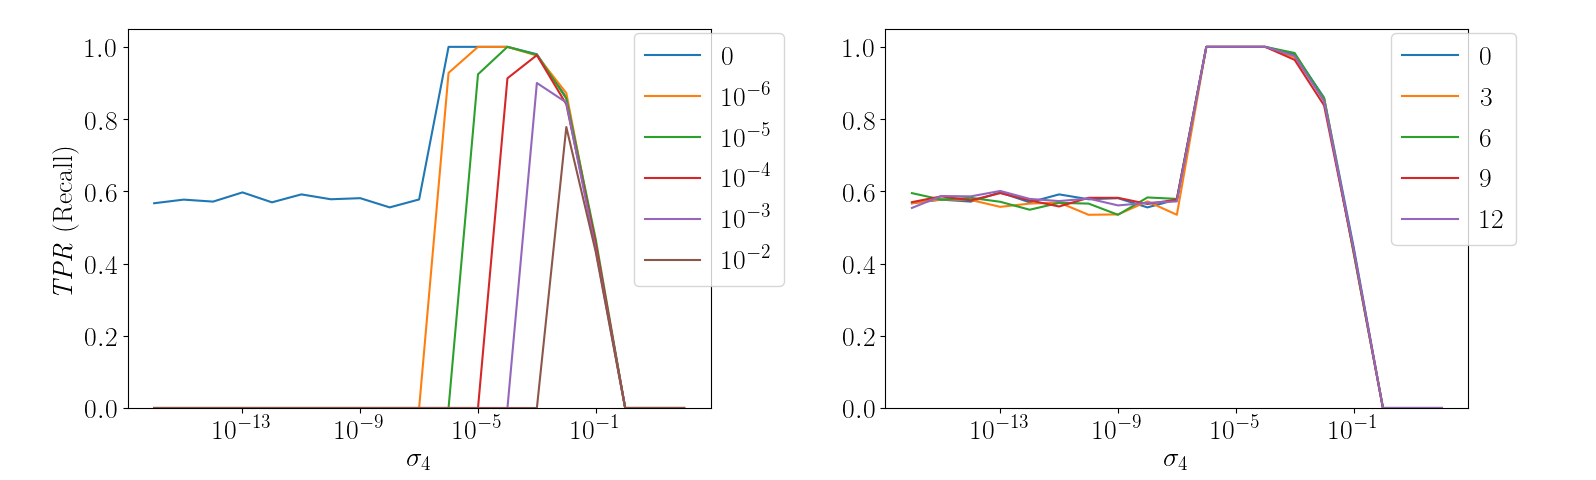
\includegraphics[scale=0.45]{images/sigma4-recall.png}
    \caption{
    Both plots depict the effect of varying $\sigma$ on the recall.
    The left plot depicts this relationship for different variations in noise, while the right plot depicts the same
    relationship for different numbers of false stars.
    The field-of-view is bounded by $f = 20^\circ$ and the apparent magnitude is bounded by $m = 6.0$.
    Each point represents the average of 200 query steps.
    } \label{figure:sigmaOverlayHyperparameterPlots}
    }
\end{figure*}

The set of plots in~\autoref{figure:sigmaOverlayHyperparameterPlots} depict the effect on different $\sigma$ terms
against the recall.
The period of accurate stability for Gaussian noise under $\sigma = 10^{-5}$ and for all false star introductions occurs
when:
\begin{equation}
    \label{eq:sigmaOverlayStableRegion}
    \sigma_4 \ \in (10^{-6}, 10^{-3})
\end{equation}

Looking at the both plots it is interesting to note that under no noise (Gaussian or false stars), a $\sigma_4 \ \in
(10^{-17}, 10^{-6})$ gives a recall of $~0.57 \pm 1.8 \times 10^{-2}$.
In this region, it appears that the \ldots
On the other end of the stability period for $\sigma_4 > 10^0$, accuracy drops straight to 0 regardless of the noise
presented.
At this period, stars are labeled with more weight to the order of the stars in the image rather than actually falling
within the specified deviation.

Focusing on the left plot of varying Gaussian noise, the accuracy dips to zero once the deviation of Gaussian noise
exceeds the selected deviation.
Past the $10^{-4}$ mark, the largest accuracy a deviation choice can achieve is no longer equal to one.
If noise is known, then the appropriate deviation for the \Call{FPO}{} method can be selected.
The right plot shows that the accuracy is not affected under different amounts of false stars.
Given varying amounts of false stars, virtually none of these stars were identified as an actual star.
The \Call{FPO}{} method is seen as highly specific, yielding no false positives.

The value of $\sigma_4 = 10^{-4}$ was selected for use in the \Call{FPO}{} method.
This is the largest deviation that lies in the accurate stable region.

\subsection{Query Selectivity}\label{subsec:querySelectivityResults}
Using the optimal hyperparameters described in the previous section, each query step was analyzed in terms of its
$Q$ and $S$ response to an introduction of Gaussian noise.

\begin{table}
    \centering {
    \caption{
    Each method's probability that the correct star set exists after querying ($Q$), average candidate set size ($S$),
    and query running time $t$ under no noise.
    Each point represents the average of 10000 query steps.
    } \label{tab:queryExperimentResults}
    \begin{tabular}{m{0.18\columnwidth}|m{0.2\columnwidth}|m{0.2\columnwidth}|m{0.2\columnwidth}}
        \textbf{Method} & $Q$ & $S$ & $t \ (ms)$  \\
        \hline \hline
        \textbf{Angle} & 1.00 & 10.666 & 68.456 \\ \hline
        \textbf{Dot Angle} & 1.00 & 1.383 & 111.474 \\ \hline
        \textbf{Spherical \newline Triangle} & 1.00 & 1.010 & 69.127 \\ \hline
        \textbf{Planar \newline Triangle} & 1.00 & 1.005 & 69.273 \\ \hline
        \textbf{Pyramid} & 0.99 & 1.325 & 70.080
    \end{tabular}
    }
\end{table}

In~\autoref{tab:queryExperimentResults}, each method's $Q, S, \text{ and } t$ is displayed without the presence of
noise.
Given that no noise is included, it is expected that all methods have 100\% accuracy- but the Pyramid method's
average accuracy is consistently 0.1\% under 100\% ($0.99 \pm 0.00188\%$ for five way split of 10000 points).
There exist 80 / 10000 runs where the Pyramid method's query step does not return the correct set.
The most likely source of error here are steps 6, 7, 8 in~\autoref{algorithm:pyramidIdentification} to produce the
$T$ sets.
A trade off of space (i.e.\ a larger catalog of precomputed trios) would avoid the common stars routine at runtime,
which would reduce these steps to one and potentially increase accuracy.

The Pyramid and Angle method use the same catalog, which is $\sim$35 times as small as the triangle method's catalog.
The Angle method also involves only one image feature filter ($\theta$) to obtain the desired result, in comparison
to the two image feature filters ($a, i$) of the triangle methods.
Querying a small catalog with a single filter allows the Angle method to achieve the fastest query step of 68.456ms.
Trailing closely by an average of 0.744ms are the Spherical and Planar Triangle methods.

Even though the Pyramid method uses the same catalog as the Angle method and only requires a single image feature
filter ($\theta$), it must perform three separate catalog accesses and find the common stars.
Consequently, in fourth place is the Pyramid method.
This method runs 0.88ms slower than the triangle average.
The Dot Angle catalog is 3 times as large as the triangle catalogs, or $\sim$105 times larger than the Angle and Pyramid
catalogs.
This query also involves three image feature filters ($\theta_1, \theta_2, \phi$) to obtain the desired result, and
as a result runs 1.6 times slower than the fastest query step (Angle method).

In terms of candidate set size, the triangle methods consistently produce the smallest average candidate set
(combined average of 1.007 sets).
For all 10000 runs, there were only 40 points for the Planar Triangle method and 63 points for the Spherical Triangle
method where the candidate set size where~\autoref{eq:nonUniqueCandidateSet} holds.
If the condition below is not true, then the reduction step can essentially be skipped (leading to faster end-to-end
runtimes).
\begin{equation}\label{eq:nonUniqueCandidateSet}
    |R| \neq 1
\end{equation}
For these 40 points of the Planar Triangle method, the average candidate set size is 2.2.
For these 63 points of the Spherical Triangle method, the average candidate set size is 2.49.
Given no noise, the planar triangle features are more distinctive than the spherical triangle features.

Third place in candidate set size is the Pyramid method, which had 2395 / 10000 points
where~\autoref{eq:nonUniqueCandidateSet}.
The average candidate set size for these 2395 points is 2.356.
In fourth place is the Dot Angle method, having 2865 points of average candidate set = 2.336 for all points where
~\autoref{eq:nonUniqueCandidateSet}.
The Pyramid method yields less sets where the query result is not unique compared to the Dot Angle method, but the
Dot Angle method produces smaller candidate sets for the points where the candidate set size is not equal to 1.

In last place by a large margin is the Angle method, which is a factor of 10 sets larger than the triangle method.
For all 10000 points, 9857 of these did not have a candidate set size equal to 1.
The Angle method has the fastest query time, but the sole image feature $\theta$ is not unique enough to identify one
star pair.

Using the measure for efficiency in~\autoref{eq:queryEfficiency}, each method ranks as follows:
\begin{multicols}{2}
    \begin{enumerate}
        \item Planar Triangle
        \item Spherical Triangle
        \item Pyramid
        \item Dot Angle
        \item Angle
    \end{enumerate}
\end{multicols}

Both the Spherical and Planar Triangle methods have the most efficient query step.

\subsection{Candidate Reduction}\label{subsec:candidateReductionResults}
Using the same optimal hyperparameters described in~\autoref{subsec:sigmaHyperparameterSelectionResults}, each query +
reduction step was analyzed in terms of the average accuracy and efficiency response to Gaussian noise and false stars.

\begin{figure*}
    \centering{
    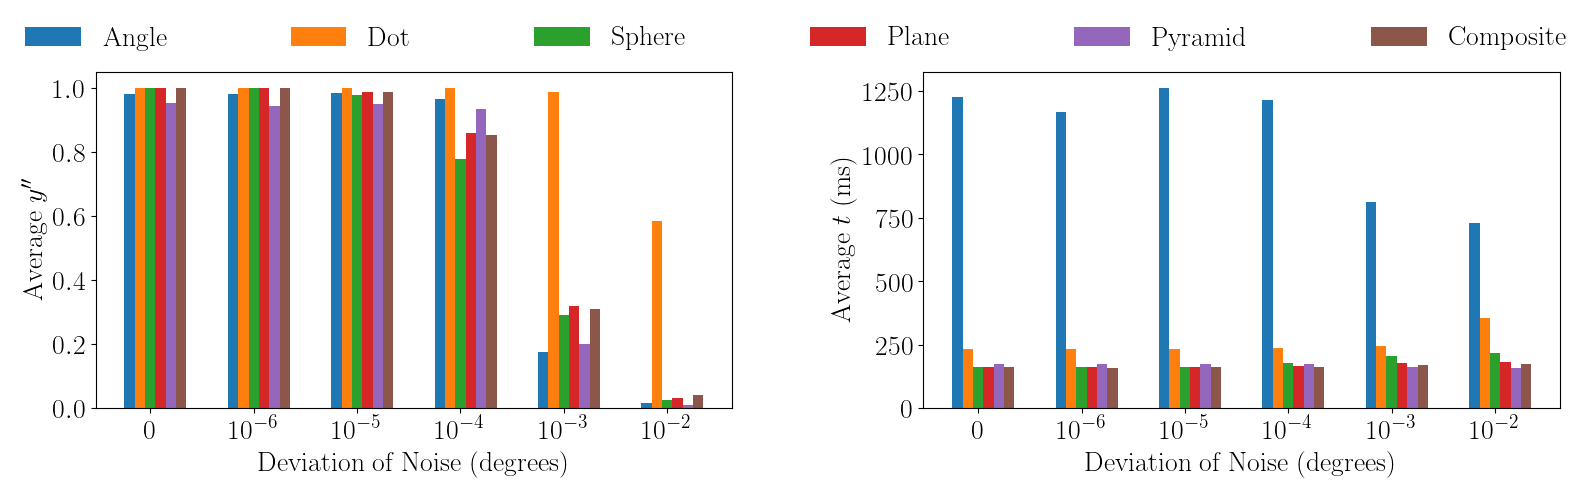
\includegraphics[scale=0.45]{images/reduction-shift-exp.png}
    \caption{
    Both plots depict the effect of varying the deviation of Gaussian noise on the average accuracy (left) and
    average running time to produce an $r$ set (right) for different identification methods.
    The field-of-view is bounded by $f = 20^\circ$ and the apparent magnitude is bounded by $m = 6.0$.
    Each method was capped at 100 query steps before erroring out and producing a false result.
    Each point represents the average and deviation of five 2000 reduction run averages.
    } \label{figure:reductionShift}
    }
\end{figure*}

Without noise in both~\autoref{figure:reductionShift} and~\autoref{figure:reductionFalse}, only the Angle method
(75\%) does not have 100\% accuracy in reduction.
The slight inaccuracies of the Pyramid method under no noise are resolved at reduction time, instead of query time
like the other methods.
In terms of speed, all methods using triangular features run on average 42.77ms faster than those using angular
features.

The Angle method has the fastest query step, but is slowed down by its $\{ R \mid 1 = |R|\}$ reduction step.
In the no noise case the Angle method is shown to have the correct candidates at query time for all runs- but
the large candidate set size at query time coupled with the single candidate set filter leads to more query-reduction
looping.
For all 10000 points in the no noise case, there only exist 143 where a sole candidate result is returned for the
first query.
Without exiting in error (> 100 query restriction), the Angle method accessed the catalog 39 times on average.
This method exited in error $\sim$25\% of the time, which accounts for all of the error observed.
Relaxing the 100 query step constraint would be beneficial toward the Angle method's accuracy at the cost of
a longer running reduction step.

The Dot Angle method is the next outlier, which also uses the $\{ R \mid 1 = |R| \}$ reduction step.
This method has 1 run out of 10000 where the number of query steps exceeds 100.
For the remaining 9999 runs, 31 of these ran for longer than 500ms (average of 1079ms runtime, 34 query steps).
The upper bound for running time is the largest of all methods, with the longest recorded running time of $\sim$3000ms.
Again, the aggressiveness of the single candidate set filter is observed here.
There exists 3625 / 10000 points where a single candidate set was returned after the first query, meaning the remaining
6375 had to perform additional queries.
If an image was encountered where $\theta_1$, $\theta_2$, and $\phi$ were not distinct enough, a large portion of time
was spent querying.
99\% of the time though, this process consumed on average 3 catalog queries to meet the single candidate set
requirement.

The 131ms average query time of the Dot Angle method is still a factor of 1.86 longer than remaining four methods.
Ranked 4th in running time is the Pyramid method, with an average query step count and running time of 1.33 steps and
76ms respectively.
The reduction step is the same as the Dot Angle and Angle method.
There exists 2432 / 10000 points where~\autoref{eq:nonUniqueCandidateSet} holds, with an average query step count of
2.4 steps.
There are slightly more cases where the query step only has to be performed once in comparison to the Dot Angle method,
but these differences magnify the flaw of the expensive Dot Angle query step.

In 1st, 2nd, and 3rd place are the Planar Triangle method, Composite Pyramid method, and Spherical Triangle method
respectively.
All of these methods have an average runtime of $68.6 \pm 0.1$ms, consuming 1 query set on average to obtain a result.
The Spherical and Planar Triangle methods use the \Call{Pivot}{} reduction step, but the majority of the $R$ reducing
comes from their efficient query steps.
For all methods combined (total of 30000 points), there exist only 144 reduction runs
where~\autoref{eq:nonUniqueCandidateSet} applied.
Of all of these, at most one additional query was required to reduce the candidate sets to a sole element.

In~\autoref{figure:reductionShift}, the deviation of Gaussian noise against the average accuracy and runtime is
displayed for different identification methods.
As soon as Gaussian noise of $10^{-5}$ degrees is introduced, all methods using triangular features can no longer
promise 100\% accuracy (average of 1.5\% decrease).
The Pyramid and Angle methods experience an average decline in accuracy of 69\% with Gaussian noise of $10^{-3}$
degrees from $10^{-4}$ degrees.
The Dot Angle method, with the largest query $\sigma$ parameter experiences a decline of 44\% with noise of $10^{-2}$
degrees from $10^{-3}$ degrees.

Note that the hyperparameters for all methods were chosen without any noise introduced.
The upper bound of the ideal region for the angular separation feature (Angle and Pyramid) was $\sigma_1 = 10^{-4}$.
The upper bound of the ideal region for the Dot Angle features was $\sigma_{(1, 2, 3)} = 10^{-2}$.
It follows that any angular noise greater than this should lead to a decline in accuracy.

For methods using triangular features, the answer is not as easy to determine.
The Planar Triangle, Spherical Triangle, and Composite Pyramid method's accuracy decreases to an average of
$73 \pm 4\%$ for noise of $10^{-4}$ degrees.
At $10^{-3}$, all triangular methods decreases to 14\%.
Beyond this, accuracy drops very close to zero (1\% at $10^{-2}$ degrees).
The triangle methods would be less sensitive to noise if the $\sigma$ parameters were increased, but this comes at the
price of time.
This can be observed with the Dot Angle method, who is able to promise near-to 100\% accuracy longer than all other
methods but has the longest query time.

Looking at the running time plot on the right, all methods except for the Dot Angle method run are fairly consistent
as noise is increased.
Intuitively, larger noise should lead to longer reduction times.
Each method's reduction step would have to iterate through more stars in the image to find the subset that fits the
reduction criteria.
The Angle method though, does not follow this reasoning.
This method actually decreases in time as $10^{-3}$ degrees of noise is introduced from $10^{-4}$ degrees, running 16ms
faster and consuming 16 less query steps.
The fact that the Angle method is taking faster to run and using less catalog accesses under more noise suggests that
the method arrives at false answers quicker than accurate ones.
Once noise goes beyond the $\sigma_1$ query parameter, the correct pair found less noisy images no longer meets the
query criteria.

As $10^{-4}$ degrees of noise is introduced, all methods using triangular features run 2.4ms longer on average.
The average query step count increase from $10^{-5}$ degrees of noise to $10^{-4}$ degrees is 36 (6.8 steps vs.
42.9 steps).
The other large jump in accuracy was observed at $10^{-3}$ degrees of noise.
From $10^{-4}$ degrees, all methods using triangular features run 1.8ms longer on average.
The average query step count increases by a factor of 1.84 here, or 36 steps.
Both the $\{ R \mid 1 = |R| \}$ and pivoting reduction step generally handle this type of noise the same.
As the noise increases with these methods, so does the number of catalog accesses and the running time.

The Dot Angle method experiences the largest jump in runtime as noise increases from $10^{-3}$ degrees to $10^{-2}$.
Runtime increases 73.7ms, and the average number of catalog accesses increases by 4.5.
For noise beyond the $\sigma_{(1, 2, 3)}$ parameters, the aggressiveness of the $\{ R \mid 1 = |R| \}$ reduction step
is seen as more iterations are required to obtain an accurate result or error out.
On the other end the Pyramid method has the most consistent running time of all methods here, running an average of
$71 \pm 1$ms for all of the trials associated with this type of noise.
From $10^{-4}$ degrees of noise to $10^{-3}$, only 1.8 more query steps are consumed on average.
From $10^{-3}$ degrees of noise to $10^{-2}$, only 1.5 more steps are consumed.

\begin{figure*}
    \centering{
    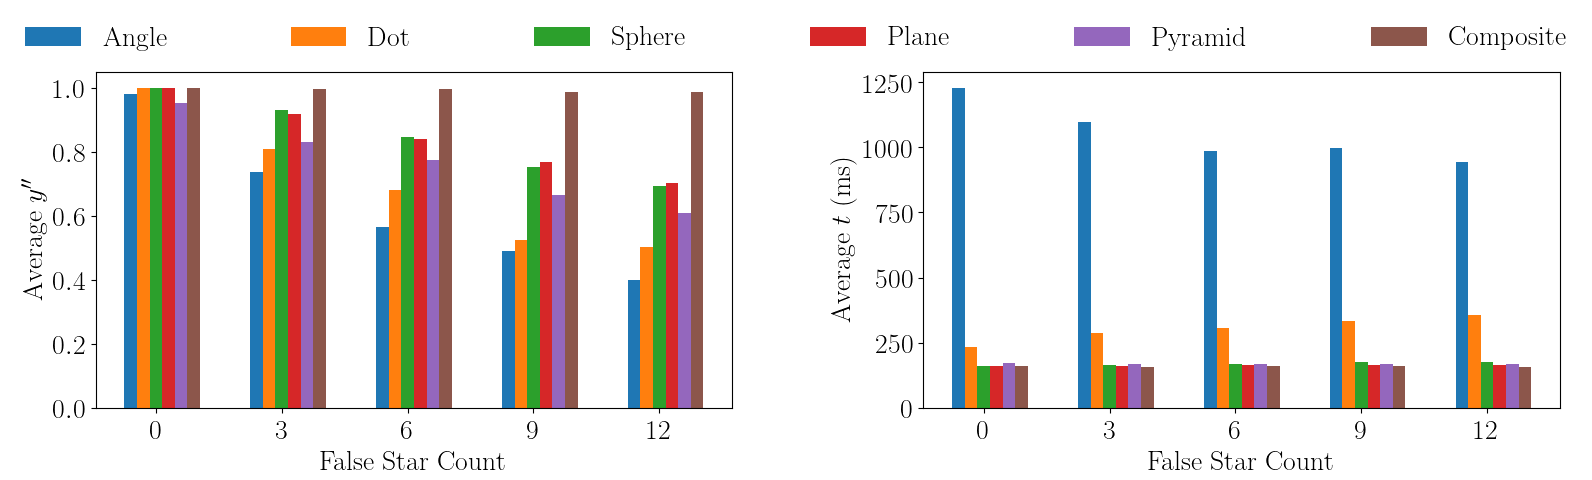
\includegraphics[scale=0.45]{images/reduction-false-exp.png}
    \caption{
    Both plots depict the effect of varying the number of false stars on the average accuracy (left) and
    average runtime to produce an $r$ set (right) for different identification methods.
    The field-of-view is bounded by $f = 20^\circ$ and the apparent magnitude is bounded by $m = 6.0$.
    Each method was capped at 100 query steps before erroring out and producing a false result.
    Each point represents the average of 10000 reduction steps.
    } \label{figure:reductionFalse}
    }
\end{figure*}

In~\autoref{figure:reductionFalse}, the number of false stars against the average accuracy and runtime is displayed
for different identification methods.
Here, all methods except for the Composite Pyramid method experience a negative accuracy response to this noise.
The list below orders each method from least responsive to most responsive from 0 to 12 false stars.
\begin{multicols}{2}
    \begin{enumerate}
        \item Composite Pyramid
        \item Planar Triangle
        \item Spherical Triangle
        \item Pyramid
        \item Angle
        \item Dot Angle
    \end{enumerate}
\end{multicols}

The Angle and Dot Angle methods experience the largest decline from no noise to 12 false stars of 42\% and 53\%
respectively.
Both methods specify no protection against this type of noise beyond the features themselves, and it follows that
both of these rank last in terms of false star tolerance.
In both~\autoref{algorithm:angleIdentification} and~\autoref{algorithm:dotAngleIdentification}, combinations are chosen
using nested loops.
An example sequence of trios (i.e.\ the three nested loop case) is depicted in~\autoref{eq:simple3NestedLoop} for
$n = 5$ stars.
\begin{equation}\label{eq:simple3NestedLoop}
a_{simple} = ( \{1,2,3\}, \{1,2,4\}, \{1,2,5\}, \{1,3,2\}, \ldots )
\end{equation}

If a false star exists in the outermost loop to produce trios, then each following $n^2$ combination will be incorrect
until the star in the outer loop changes.
This gives the Dot Angle method $n^2$ more opportunities to choose a wrong trio in this case, and is likely why it is
the most responsive to false stars.
The Angle method method only requires two nested loops, which gives only $n$ incorrect combinations if a false star
exists in the outer loop.
This higher turnover allows the Angle method to perform only slightly worse than the rest of the methods (besides
the Composite Pyramid).

The Spherical and Planar Triangle methods use the same method to choose combinations as the Dot Angle method, but differ
in their use of the \Call{Pivot}{} method and their query features.
If a false star is chosen in the outer loop for either of the triangle methods, the addition of the \Call{Pivot}{} call
gives $n^2 \times n = n^3$ more opportunities to choose the wrong trio.
Even though this is a factor of $n$ worse than the Dot Angle method, the efficiency of the query step for these
methods appear to mitigate the potential errors.

Both the Composite Pyramid and Pyramid methods specify a false star persistence avoidance process for choosing
query star sets as opposed to the simple triple nested loops of the other methods.
An example sequence of this process given an image of $n=5$ stars is depicted below.
\begin{equation}\label{eq:pyramidNestedLoop}
a_{pyramid} = ( \{1,2,3\}, \{2,3,4\}, \{3,4,5\}, \{1,2,4\}, \ldots)
\end{equation}
If star 1 was a false star in~\autoref{eq:pyramidNestedLoop}, then the next element would not use it.
This works well in increasing the accuracy of the Composite Pyramid method's reduction step, but not in the Pyramid's
reduction step.
The main difference between these two methods are their query steps, suggesting that triangular features themselves
are more tolerant to this noise than angular features.

% TODO: Finish this shitttttttt
The running time plot again shows that the Angle method runs faster when more noise is introduced.
From 0 to 12 false stars, the Angle method runs 6.0ms faster and consumes 10 less query steps on average.

If one false star exists in the selected image subset,

There are more candidate sets with false stars than
There appears to be more candidate sets with

The running time plot shows that the Dot Angle method and Pyramid method generally takes longer to run when given more
false stars, while the rest of the methods's running times are inversely proportional to the number of false stars.
The largest running time response for the Dot Angle method occurs from 3 false stars to 6 false stars, with an increase
of XXXms.
From 6 to 12 false stars, the average increase is XXXms per 3 additional false stars.
The Pyramid method has a more consistent response to running time, taking XXXms longer to run per 3 false stars.
Here, more catalog accesses are required to find a correct trio.

For the other methods, this does not appear to be the case.

In both of these methods, more catalog accesses are required to find a corrrect trio

\subsection{Identification Determination}\label{subsec:identificationDeterminationResults}
Using all optimal hyperparameters described in~\autoref{subsec:sigmaHyperparameterSelectionResults}, each identification
was ran end-to-end and analyzed in terms of its response to an introduction of Gaussian noise and false stars.

\begin{figure*}
    \centering{
    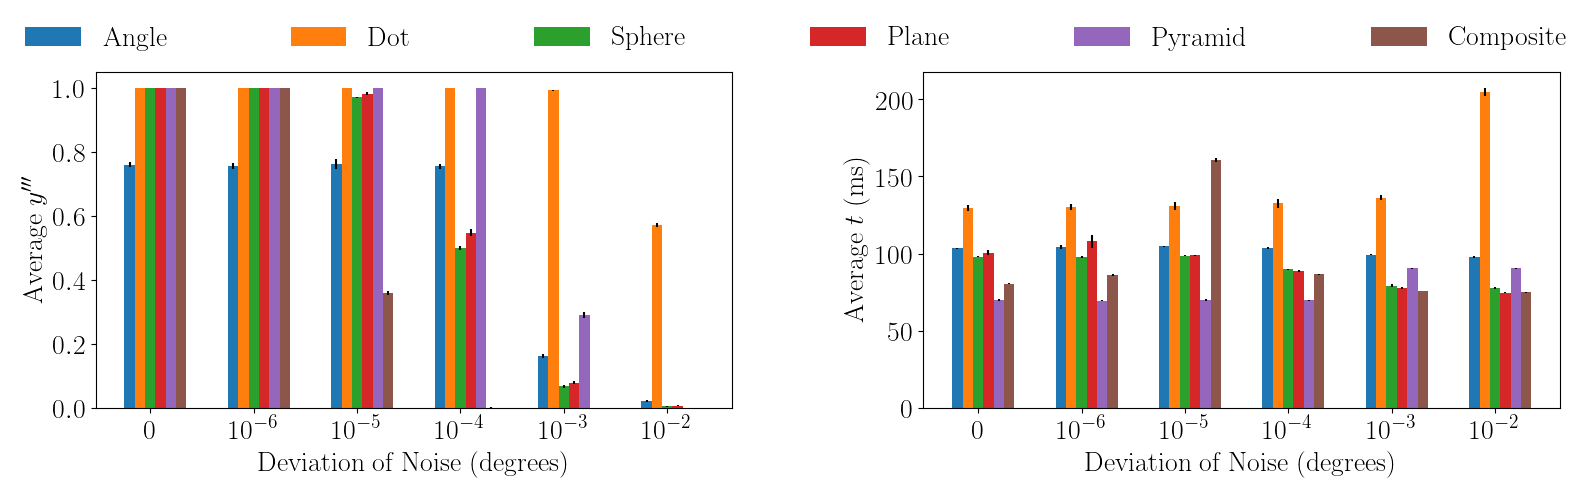
\includegraphics[scale=0.45]{images/identification-shift-exp.png}
    \caption{
    Both plots depict the effect of varying the deviation of noise on the average accuracy (left) and average
    running time to produce a map $a$ (right) for different identification methods.
    The field-of-view is bounded by $f = 20^\circ$ and the apparent magnitude is bounded by $m = 6.0$.
    Each method was capped at 100 query steps before erroring out and producing a false result.
    Each point represents the average of 10000 identification steps.
    } \label{figure:identificationShift}
    }
\end{figure*}

%Without noise in both~\autoref{figure:identificationShift} and~\autoref{figure:identificationFalse}, all methods except
%for the Angle and Composite Pyramid yield 100\% accuracy.
%Out of these 100\% accuracy methods, the Pyramid method had the shortest running time here, running an average of
%214ms to obtain a result.
%The Dot Angle method is 2nd in this group, requiring 8.5s to obtain a result.
%The Spherical and Planar Triangle methods follow here, running an average of 14.2s to obtain a correct result.
%Out of the two methods that are not 100\% accurate under no noise (Angle, Composite Pyramid), the Angle ran the fastest.
%The Composite Pyramid took the longest to run, at 324s to obtain a result.
%
%Comparing the results found in reduction experiment without noise to these results here, the Pyramid and Dot Angle
%methods rely on the~\autoref{figure:genericIdentificationMethodFlowchart} filter after the reduction step to boost
%its accuracy to 100\%.
%The Angle method shows no difference in accuracy here, but the Composite Pyramid method appears to decline from 64\%
%to 44\%.
%Given that all triangle methods use the \Call{DMT}{} call in its identification step, the culprit here appears to be
%from the \Call{VerifyC}{} procedure.
%This may be another strong filter that is hindering the performance of the Composite Pyramid method, similar to its
%reduction step.
%
%In~\autoref{figure:identificationShift}, the deviation of Gaussian noise is displayed against the average accuracy and
%running time.
%When noise of $10^{-5}$ degrees is introduced, the same decline in accuracy as seen in the reduction experiment can be
%seen here.
%All methods using triangular features decline to an average accuracy of 31\%.
%The identification step of all triangular feature methods involve the \Call{DMT}{} procedure.
%Inaccuracies in this procedure can be found by subtracting the accuracies found in the reduction
%experiment by those found here.
%This average difference is 10\%, suggesting that the \Call{DMT}{} call does account for some of the additional
%inaccuracy.
%
%When noise of $10^{-3}$ degrees is introduced, all methods with angular features decline to an average accuracy of
%18\%.
%This is where all angular methods sharply dropped in accuracy for the reduction experiment, and it follows that the
%accuracy in the previous steps should affect the future steps (identification).
%For the Angle method, the \Call{DMT}{} call is another limiting factor for accuracy.
%Recall that the $\sigma$ value chosen for the \Call{FPO}{} procedure was $10^{-4}$.
%Any differences beyond the overlay $\sigma$ will not be counted, and the \Call{DMT}{} call will have less
%information to work with.
%
%The Dot Angle method shows no difference between its reduction accuracy and identification accuracy.
%This method determines the $a$ map at query time, and it follows that no additional inaccuracies can occur after
%reduction.
%The Pyramid method has a higher accuracy than its reduction results, showing that the \textit{Confident in $r$?} filter
%is fairly effective.
%This method is the most accurate and quickest under the most noise ($10^{-3}$ degrees), requiring roughly 193ms to
%run from start to finish.
%
%The only methods that appear to have a significant running time response to noise are those with triangular features.
%Given that these methods have the most expensive query (at 12.7s per query), any additional queries will be penalized.
%The average increase in running time for the Spherical and Planar Triangle methods with images of no noise to those with
%$10^{-3}$ degrees of noise is 216s.
%For the Composite Pyramid, there appears to be decrease in running time as the noise increases (decrease of 90s from
%no noise to $10^{-3}$ degrees of Gaussian noise).
%The Angle method is the 2nd fastest identification method (285ms), followed by the Dot Angle method (7.7s).

%In~\autoref{figure:identificationFalse}, the number of false stars against the average accuracy and runtime is
%displayed for different identification methods.
%In 1st place again, with close to 100\% accuracy given any number of false stars is the Pyramid method.
%The effectiveness of the false star persistence avoidance process combined with the \textit{Confident in $r$?} filter
%shines here.
%This same false star persistence avoidance process might also attribute to the Composite Pyramid not declining in
%accuracy as much as the other methods (but it still does decline).
%
%All other methods (Spherical / Planar Triangle, Angle, Dot Angle) appear to decline to the same accuracy at 35\%
%given 12 false stars, indicating that choosing query steps is vital in properly handling false stars.
%For all of these methods a false star is for the outer loop means iterating through every combination of stars with
%this false star.
%Any result that is returned from here to the next iteration of the outer loop will be false, and it is important to
%cycle through as many unique image star sets as possible to avoid this problem.
%
%As the number of false stars increases, the running time increases for the Spherical and Planar triangle methods.
%For each three false star increment, there is an average of 40s increase in running time.
%
%For the other methods, there does not appear to be a response to running time here as the number of false stars
%increases.
%In order of shortest running time, each method ranks as follows:
%\begin{multicols}{2}
%    \begin{enumerate}
%        \item Pyramid
%        \item Angle
%        \item Dot Angle
%        \item Planar Triangle
%        \item Spherical Triangle
%        \item Composite Pyramid
%    \end{enumerate}
%\end{multicols}
%
%The Pyramid method is ~1500 as fast as the Composite Pyramid method, requiring an average of 211ms to present a result
%given an image of 12 false stars.
%The Angle method is a close 2nd place, with an average running time of 240ms.
%Distant from 2nd place and 4th is the Dot Angle method, with an average running time of 6.7s.
%The Spherical and Planar Triangle methods require an average of 107s to produce a result.
%
%The Pyramid method is the best identification method for handling images with both types of noise, and is also the
%most efficient.

\begin{figure*}
    \centering{
    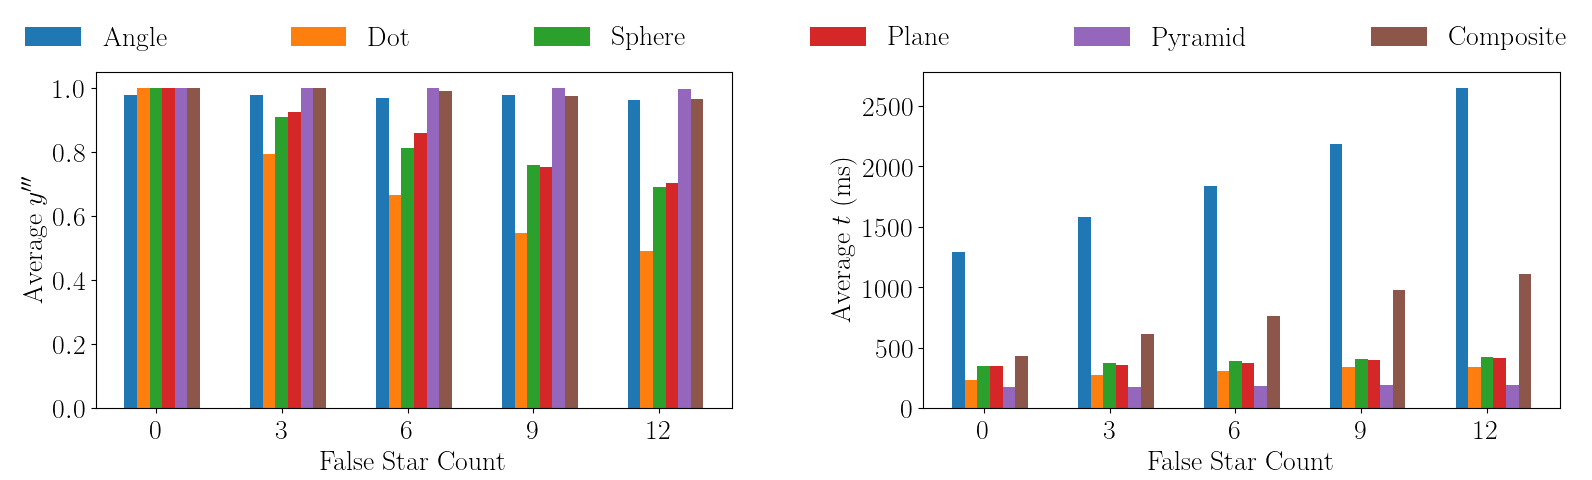
\includegraphics[scale=0.45]{images/identification-false-exp.png}
    \caption{
    Both plots depict the effect of varying the number of false stars on the average accuracy (left) and average running
    time to produce a map $a$ (right) for different identification methods.
    The field-of-view is bounded by $f = 20^\circ$ and the apparent magnitude is bounded by $m = 6.0$.
    Each method was capped at 100 query steps before erroring out and producing a false result.
    Each point represents the average of 10000 identification steps.
    } \label{figure:identificationFalse}
    }
\end{figure*}
